Para algunos administradores de Bases de datos y desarrolladores, optimizar las consultas es la parte más importante de la optimización de una base de datos. 

\section{Data de ejemplo}

Para optimizar consultas, se necesita data que analizar, para lo cual se utilizará la base de datos \textbf{Dell Store 2}, originalmente creata por Dell y luego portada a PostgreSQL. Se puede descargar de \emph{http://pgfoundry.org/projects/dbsamples/}.\\

\emph{\$ wget http://pgfoundry.org/frs/download.php/543/dellstore2-normal-1.0.tar.gz\\
\$ tar xvfz dellstore2-normal-1.0.tar.gz\\
\$ cd dellstore2-normal-1.0/\\
\$ sudo su postgres -c``createdb dellstore2''\\
\$ sudo su postgres -c ``psql -f dellstore2-normal-1.0.sql -d dellstore2''\\
\$ sudo su postgres -c ``psql -d dellstore2 -c ``VACUUM VERBOSE ANALYZE''''\\
}

Para conocer el tamaño de la base de datos ejecutar:\\

\begin{pyglist}
SELECT pg_size_pretty(pg_database_size('dellstore2'));
\end{pyglist}

Los ejemplos en este capítulo se darán a partir de \textit{Dell Store 2}, a menos que se indique lo contrario. \cite{GregorySmith2010}\\

La estructura de la data es sencilla:

\begin{itemize}
\item Hay un número de productos que la tiendas vende, cada uno de los cuáles entra en una categoría.
\item La tienda tiene clientes.
\item Los clientes dan órdenes de compra.
\item Cada orden tiene un número de líneas, cada una de las cuáles referencia productos siendo comprados.
\item Una historia de cliente es salvada listando todos los productos que el cliente alguna vez ha ordenado.
\end{itemize}

\section{Timing}

Para conocer cuanto demora en ejecutarse una consulta se utiliza el comando timing antes de ejecutar la consulta de tal manera que mida el tiempo requerido.\\

\begin{pyglist}
dellstore2=# \timing
dellstore2=# SELECT count(*) FROM customers;
count 
------- 
20000 
Time: 9,245 ms
\end{pyglist}

Para desactivar volver a escribir $\backslash$timing.

\section{Explain y Explain Analyze}

Para conocer el porque de velocidad de ejecución de una consulta se utiliza el comando EXPLAIN antes de la consulta lo cual muestra el resultado esperado de dicha consulta o query plan (plan de la consulta).\\

Si se utiliza EXPLAIN ANALYZE se obtiene la estimación describiendo lo que espera el planificador de PostgreSQL y además lo que realmente sucede después de ejecutar la consulta.\\

Por ejemplo, si se ejecuta:\\

\begin{pyglist}
EXPLAIN ANALYZE DELETE * FROM t;
\end{pyglist}

No solo se va a obtener el plan sino efectivamente se va a eliminar todo el contenido de la tabla t.

\section{Las consultas y la cache}

Cuando la data necesaria para responder a una consulta está en la cache de la base de datos o del sistema operativo, la consulta se lleva a cabo más rápido debido a que ya no se necesita recuperar la data del disco, solo obtenerla de la memoria.\\

Si se ejecuta dos veces una consulta, la segunda vez va a ejecutarse más rápido. Cuando la consulta empieza a ejecutarse siempre con la misma duración, significa que su data en la cache se ha estabilizado y ya no indice en el resultado. \cite{GregorySmith2010}

\subsection{Efecto de la cache}

Para identificar el impacto de la cache, se va a limpiar la cache del sistema y luego se volverá a ejecutar la consulta:\\

Limpiar la cache:\\

\emph{
 \$ sudo /etc/init.d/postgresql stop \\
 \$ sudo su \\
 \# sync \\
 \# echo 3 > /proc/sys/vm/drop\_caches \\
 \# exit\\
 \$ sudo /etc/init.d/postgresql start\\
 }
 
Se ejecuta la consulta:\\

\emph{\$ psql -d dellstore2}

\begin{pyglist}
\timing
SELECT count(*) FROM customers;
 count 
-------
 20000
(1 fila)

Duracion: 350,276 ms

SELECT count(*) FROM customers;
 count 
-------
 20000
(1 fila)
\end{pyglist}

Como se puede apreciar, la cache influencia en gran medida el rendimiento de las consultas en el sistema. Para eliminar el efecto de la cache sobre una consulta, esta debe ser ejecutada varias veces hasta que sus tiempo de ejecución sean similares.

\subsection{Estructura del plan de la consulta}

La salida del comando EXPLAIN está organizada en una serie de nodos. Cada línea de la salida es un nodo. Al más bajo nivel están los nodos que analizan tablas e índices. Los nodos de más alto nivel cogen la salida de los nodos de bajo nivel y operan sobre esta.\\

Por ejemplo:\\

\begin{pyglist}
# EXPLAIN ANALYZE SELECT * FROM customers;
QUERY PLAN                                                   
----------------------------------------------------------------------------------------------------------------
 Seq Scan on customers  (cost=0.00..676.00 rows=20000 width=268)
  (actual time=0.010..27.434 rows=20000 loops=1)
 Total runtime: 52.451 ms
(2 filas)
\end{pyglist}

Al ejecutarse con \textit{EXPLAIN ANALYZE} la duración aumenta varias veces. En casos de querys más complejos la sobrecarga producida por el análisis es menor, aún así no se debe de confiar completamente en los tiempo producidos por \textit{EXPLAIN ANALYZE}.\\

Este plan tiene un nodo, un nodo \textit{Seq Scan}

\begin{itemize}
\item cost=0.00..676.00: El primer costo es el costo de iniciar el nodo. Esto es cuanto trabajo es estimado antes de que este nodo produzca su primera fila de salida. En este caso es 0 ya que una búsqueda secuencial devuelve resultados de forma inmediata. El segundo número es el costo estimado de ejecutar todo el nodo hasta que termine.
\item rows=20000:  El número de filas que este nodo espera como salida.
\item width=268 : El número esperado de bytes de cada fila de la salida. 
\end{itemize}

Los números actuales muestran como realmente se llevo a cabo la consulta:
\begin{itemize}
\item actual time=0.011..34.489: El actual costo de inicio no fue cero, se necesito una pequeña fracción de tiempo para empezar. Una vez que empezó necesito 34.489 segundos para terminar.
\item Rows=20000: Tal como se esperaba fueron 20000 filas.
\item loops=1: Algunos nodos, como los que hacen joins, se ejecutan más de una vez. En ese caso el valor de loops va a ser más de uno y el tiempo y la cantidad de filas van a ser referidas a cada loop no al total.
\end{itemize}

\subsection{Costo de computación}

La labor básica del optimizador de consultas es generar planes que puedan utilizarse para ejecutar una consulta y escoger el que tenga el menor costo de ejecución. El costo es hecho de forma arbitraria.

\begin{itemize}
\item seq\_page\_cost: Cuanto demora leer una sola página desde el disco en forma secuencial. El resto de parámetros son relativos a este cuyo valor es 1.0.
\item random\_page\_cost: El costo de lectura cuando los registros están dispersos por varias páginas. El valor por defecto es 4.0.
\item cpu\_tuple\_cost: Cuanto cuesta procesar un solo registro, su valor por defecto 0.1.
\item cpu\_index\_tuple\_cost: El costo de procesar una sola entrada de un índice. El valor por defecto es 0.005, menor de lo que cuesta procesar un registro debido a que los registros tienen mucha más información de cabecera (como \textit{xmin} y \textit{xmax}).
\item cpu\_operator\_cost: El costo esperado de procesar una función o un operador (la suma de dos números por ejemplo) y por defecto es 0.0025.
\end{itemize}

Se puede comparar en una tabla:\\

\begin{table}[h]
\centering
\begin{tabular}{|c|c|c|} \hline
Parámetro             & Valor por Defecto & Velocidad relativa    \\ \hline
seq\_page\_cost         & 1.0               & Reference \\ \hline
random\_page\_cost      & 4.0               & 4X slower \\ \hline
cpu\_tuple\_cost        & 0.01              & 100X faster\\ \hline     
cpu\_index\_tuple\_cost  & 0.005             & 200X faster \\ \hline
cpu\_operator\_cost     & 0.0025            & 400X faster \\ \hline
\end{tabular}
\end{table}

Todos estos valores se pueden encontrar en \textit{postgresql.conf}.\\

Se pueden utilizar estos números para calcular el costo mostrado en el ejemplo previo. Una búsqueda secuencial de la tabla ``customers'' debe leer cada página en la tabla y procesar cada registro. Se pueden combinar los costos internos utilizados por PostgreSQL con las estadísticas utilizadas por el optimizador.\\

\begin{pyglist} 
SELECT
relpages,
current_setting('seq_page_cost') AS seq_page_cost,
relpages *
current_setting('seq_page_cost')::decimal AS page_cost,
reltuples,
current_setting('cpu_tuple_cost') AS cpu_tuple_cost,
reltuples *
current_setting('cpu_tuple_cost')::decimal AS tuple_cost
FROM pg_class WHERE relname='customers';
\end{pyglist}

Se obtiene:\\

\begin{pyglist} 
relpages | seq_page_cost | page_cost | reltuples | cpu_tuple_cost | tuple_cost  
----------+---------------+-----------+-----------+----------------+------------ 
      476 | 1             |       476 |     20000 | 0.01           |        200 
\end{pyglist}

Agregar el costo de leer la página (\textit{page\_cost}) al costo de procesar los registros (\textit{tuple\_cost}) y se obtiene 676, el costo mostrado por \textit{EXPLAIN}.\\

Los parámetros de costo se pueden configurar, una configuración común cuando se sabe que gran parte de la base de datos puede entrar en la memoria es reducir \textit{random\_page\_cost} a 2, debido a que un elevado porcentaje de las páginas está en la cache y es encontrada con mayor facilidad que en el disco.\\

Para saber que columnas se están utilizando en una consulta, se puede utilizar el modo verboso:\\

\begin{pyglist}
EXPLAIN VERBOSE SELECT * FROM customers;
\end{pyglist}

\section{Optimización de consultas}

Para optimizar las consultas en primer lugar se explicará como mejorar el rendimiento de la obtención de los registros y luego de las operaciones con los registros.

\subsection{Armando conjuntos de registros}

Para optimizar la selección de los registros buscados por una consulta se pueden tomar en cuenta diversas optimizaciones.

\subsubsection{Id de los registros}

Todo registro tiene un Id, el que se puede ver en la columna \textit{ctid}. Se puede utilizar en una misma transacción para referirse a un registro que se repite varias veces y así acelerar su búsqueda. No es útil en diferentes transacciones ya que puede cambiar con una actualización. También sirve para distinguir entre registros idénticos, por ejemplo al eliminar registros duplicados.\\

Un ejemplo de ctid:\\

\begin{pyglist}
EXPLAIN SELECT customerid FROM customers WHERE ctid='(0,1)';

                       QUERY PLAN                        
---------------------------------------------------------
 Tid Scan on customers  (cost=0.00..4.01 rows=1 width=4)
   TID Cond: (ctid = '(0,1)'::tid)
\end{pyglist}

\subsubsection{Índices}

Cuando se ejecutan consultas que incluyen LIMIT es útil buscar mediante un campo que este indexado, ya que así el ordenamiento será más rápido.

\subsection{Procesando los nodos} 

Una vez que se tiene un conjunto de registros, el siguiente tipo de nodo que se va a encontrar cuando se usa una sola tabla son aquellos que procesan el conjunto de varias formas. Estos nodos por lo general cogen un conjunto de registros y devuelven otro.

\subsubsection{Ordenamiento - Sort}

Nodos de ordenamiento aparecen cuando se utiliza \textit{ORDER BY} en las consultas:\\

\begin{pyglist}
 EXPLAIN ANALYZE SELECT customerid FROM customers ORDER BY zip;
                                    QUERY PLAN                                                     
-----------------------------------------------------------------------
 Sort  (cost=2104.77..2154.77 rows=20000 width=8) 
        (actual time=74.299..101.232 rows=20000 loops=1)
   Sort Key: zip
   Sort Method: external sort  Disk: 352kB
   ->  Seq Scan on customers  (cost=0.00..676.00 rows=20000 width=8)
    (actual time=0.013..33.266 rows=20000 loops=1)
 Total runtime: 126.535 ms
\end{pyglist}

Las operaciones de ordenamiento se pueden ejecutar en memoria (más rápido) o en disco (más lento). En el ejemplo podemos ver que a pesar de la pequeña cantidad de data (352kB) esta ha sido calculada en el disco. Aún cuando es menor que el valor por defecto de \textit{work\_mem} (1MB), el algoritmo quicksort (utilizado en la memoria) necesita más memoria que la utilizada en el disco duro al combinar archivos previamente ordenados. Si el parámetro \textit{work\_mem} es incrementado, la operación se lleva a cabo en memoria. \cite{GregorySmith2010}\\

\begin{pyglist}
SET work_mem='2MB';
EXPLAIN ANALYZE SELECT customerid FROM customers ORDER BY zip;
                                   QUERY PLAN                                                     
-----------------------------------------------------------------------------
 Sort  (cost=2104.77..2154.77 rows=20000 width=8)
      (actual time=62.513..87.639 rows=20000 loops=1)
   Sort Key: zip
   Sort Method: quicksort  Memory: 1294kB
   ->  Seq Scan on customers  (cost=0.00..676.00 rows=20000 width=8) 
                     (actual time=0.015..31.845 rows=20000 loops=1)
 Total runtime: 112.588 ms
\end{pyglist}

Se puede apreciar que el valor por defecto no era suficiente y se necesitaba aumentar \textit{work\_mem} para que la operación se llevara a cabo en la memoria.\\

\subsubsection{Funciones de agregación - Aggregate}

Las funciones de agregación reciben una serie de valores y producen una sola salida. Algunos ejmeplos son AVG(), COUNT(), EVERY(), MIN(), MAX(), STDDEV() y SUM(). Para calcular una función de agregación, se leen todos los registros y luego se pasan por por el nodo agregado para calcular el resultado:\\

\begin{pyglist}
EXPLAIN ANALYZE SELECT max(zip) FROM customers;
                                   QUERY PLAN                                                     
------------------------------------------------------------------------
 Aggregate  (cost=726.00..726.01 rows=1 width=4) 
 (actual time=56.127..56.128 rows=1 loops=1)
   ->  Seq Scan on customers  (cost=0.00..676.00 rows=20000 width=4) 
                       (actual time=0.011..26.958 rows=20000 loops=1)
 Total runtime: 56.203 ms
\end{pyglist}

No siempre este el caso, al utilizar índices el tiempo disminuye considerablemente:\\

\begin{pyglist}
EXPLAIN ANALYZE SELECT max(customerid) FROM customers;
   QUERY PLAN                                                                         
----------------------------------------------------------------------
 Result  (cost=0.03..0.04 rows=1 width=0)
       (actual time=0.064..0.066 rows=1 loops=1)
   InitPlan 1 (returns $0)
     ->  Limit  (cost=0.00..0.03 rows=1 width=4) 
          (actual time=0.054..0.056 rows=1 loops=1)
           ->  Index Only Scan Backward using customers_pkey on customers 
               (cost=0.00..534.25 rows=20000 width=4) 
               (actual time=0.049..0.049 rows=1 loops=1)
                 Index Cond: (customerid IS NOT NULL)
                 Heap Fetches: 0
 Total runtime: 0.120 ms $
\end{pyglist}

\subsection{Joins}

Las tareas más complejas del planificador de consultas son las que tienen que ver con unir tablas entre si. Cada vez que se agrega una tabla al conjunto que se le aplicará join, el número de posibilidades crece de forma dramática. Si solo son tres tablas, el planificar considerará todo posible plan para seleccionar el óptimo, pero si son veinte tablas, la cantidad de posibilidades es muy grande para considerarlas todas. \cite{GregorySmith2010}\\

En un \textit{CROSS JOIN} se multiplican todos los registros de una tabla por los de otra, multiplicando de forma anidada cada registro por toda la otra tabla. En pseudocódigo:\\

\begin{pyglist}
for each outer row:
    for each inner row:
        if join condition is true:
           output combined row
\end{pyglist}

Se puede observar algo similar en data real si es que se unen dos tablas sin un \textit{WHERE} de por medio.

\begin{pyglist}
EXPLAIN ANALYZE SELECT * FROM products,customers;
                      QUERY PLAN                                                        
--------------------------------------------------------------------------
 Nested Loop  (cost=0.00..2500899.00 rows=200000000 width=317) 
              (actual time=17.844..791143.955 rows=200000000 loops=1)
   ->  Seq Scan on customers  (cost=0.00..676.00 rows=20000 width=268)
                  (actual time=9.394..102.243 rows=20000 loops=1)
   ->  Materialize  (cost=0.00..248.00 rows=10000 width=49)
              (actual time=0.002..12.694 rows=10000 loops=20000)
         ->  Seq Scan on products  (cost=0.00..198.00 rows=10000 width=49) 
                          (actual time=8.411..25.013 rows=10000 loops=1)
 Total runtime: 1029182.979 ms

\end{pyglist}


\subsubsection{Bucle anidado con búsqueda mediante índices} 

Lo más común en un bucle anidado donde una tabla solo está devolviendo un número limitado de registros. Si existe un índice en una de las tablas, el optimizador lo utilizará para limitar el número de registros y hacer el tiempo de ejecución menor.\\

Considerar el caso donde se está buscando una sola orden utilizando un campo sin índice (por lo que la búsqueda debe ser secuencial) pero haciendo un join con su respectiva orden de compra.\\

\begin{pyglist}
EXPLAIN ANALYZE SELECT * FROM orders,orderlines WHERE 
orders.totalamount=329.78 AND orders.orderid=orderlines.orderid;

QUERY PLAN                                                                
-----------------------------------------------------------------------
 Nested Loop  (cost=0.00..259.41 rows=5 width=48) 
              (actual time=0.070..8.387 rows=9 loops=1)
   ->  Seq Scan on orders  (cost=0.00..244.00 rows=1 width=30) 
                      (actual time=0.047..8.316 rows=1 loops=1)
         Filter: (totalamount = 329.78)
         Rows Removed by Filter: 11999
   ->  Index Scan using ix_orderlines_orderid on orderlines  
     (cost=0.00..15.36 rows=5 width=18) 
                  (actual time=0.012..0.029 rows=9 loops=1)
         Index Cond: (orderid = orders.orderid)
 Total runtime: 8.472 ms
\end{pyglist}

En caso de que ambas tablas utilicen un índice la consulta es aún más rápida:\\

\begin{pyglist}
EXPLAIN ANALYZE SELECT * FROM orders,orderlines WHERE orderlines.
orderid=1000 AND orders.orderid=orderlines.orderid;

 QUERY PLAN                                                                
------------------------------------------------------------------------------
 Nested Loop  (cost=0.00..23.66 rows=5 width=48) 
              (actual time=0.048..0.087 rows=6 loops=1)
   ->  Index Scan using orders_pkey on orders  (cost=0.00..8.27 rows=1 width=30) 
                                       (actual time=0.026..0.029 rows=1 loops=1)
         Index Cond: (orderid = 1000)
   ->  Index Scan using ix_orderlines_orderid on orderlines  
                                               (cost=0.00..15.34 rows=5 width=18)
                                       (actual time=0.011..0.025 rows=6 loops=1)
         Index Cond: (orderid = 1000)
 Total runtime: 0.173 ms
\end{pyglist}


\subsubsection{Merge Join}

Este tipo de join requiere que ambas entradas esten ordenadas, luego busca a través de las dos en orden moviendose un registro a la vez a través de las tablas mientras los valores las columnas utilizadas para el join cambian. Una tabla puede ser revisada varias veces si la tabla por la que se busca tiene valores repetidos.\\

Para ver un merge join se necesita una condición de igualdad como la mostrada en un reporte donde se indica cuanto ha comprado cada cliente:\\

\begin{pyglist}
EXPLAIN ANALYZE SELECT C.customerid,sum(netamount) FROM customers C,
orders O WHERE C.customerid=O.customerid GROUP BY C.customerid;

QUERY PLAN                                                                        
-----------------------------------------------------------------
 GroupAggregate  (cost=0.03..1536.49 rows=12000 width=10) 
           (actual time=28.443..176.144 rows=8996 loops=1)
   ->  Merge Join  (cost=0.03..1356.49 rows=12000 width=10)
                       (actual time=28.420..142.030 rows=12000 loops=1)
         Merge Cond: (c.customerid = o.customerid)
         ->  Index Only Scan using customers_pkey on customers c 
                               (cost=0.00..484.25 rows=20000 width=4) 
                      (actual time=28.358..56.956 rows=20000 loops=1)
               Heap Fetches: 0
         ->  Index Scan using ix_order_custid on orders o  
                               (cost=0.00..672.24 rows=12000 width=10) 
                             (actual time=0.021..25.228 rows=12000 loops=1)
 Total runtime: 187.058 ms
\end{pyglist}

La consulta se realiza siguiendo los índices de \textit{customerid} tanto en \textit{customers} como en \textit{orders} para encajar ambas tablas entre si de forma ordenada. Luego el ejecutor puede utilizar un Merge Join de forma eficiente para combinar ambos.\\

Para optimizar esta consulta es útil no hacer el join con campos cuyas columnas tengan tablas repetidas.

\subsubsection{Hash Join}

La principal alternativa utilizada por PostgreSQL para un Merge Join es un Hash Join. Este tipo de Join no ordena sus entradas, en vez de eso, crea una tabla Hash para cada registro de una tabla con los registros correspondientes de la otra tabla. La salida no necesariamente va a estar en orden.\\

Una consulta para encontrar los productos que en algún punto han sido ordenados por cualquier cliente muestra un Hash Join.\\

\begin{pyglist}
EXPLAIN ANALYZE SELECT prod_id,title FROM products p WHERE EXISTS 
(SELECT 1 FROM orderlines ol WHERE ol.prod_id=p.prod_id);

 QUERY PLAN                                                             
------------------------------------------------------------------
 Hash Join  (cost=1328.43..1773.80 rows=9736 width=19) 
           (actual time=216.478..260.593 rows=9973 loops=1)
   Hash Cond: (p.prod_id = ol.prod_id)
   ->  Seq Scan on products p  (cost=0.00..198.00 rows=10000 width=19)
                         (actual time=0.008..13.163 rows=10000 loops=1)
   ->  Hash  (cost=1206.73..1206.73 rows=9736 width=4) 
                       (actual time=216.436..216.436 rows=9973 loops=1)
         Buckets: 1024  Batches: 1  Memory Usage: 234kB
         ->  HashAggregate  (cost=1109.38..1206.73 rows=9736 width=4)
                      (actual time=187.953..202.345 rows=9973 loops=1)
           ->  Seq Scan on orderlines ol (cost=0.00..958.50 rows=60350 width=4)
                                 (actual time=0.008..91.152 rows=60350 loops=1)
 Total runtime: 272.643 ms

\end{pyglist}
           
Dependiendo del tipo de entrada puede ser mejro o peor que Merge Join. Si la entrada no está ordenada puede ser mejor que el Merge Join. Además, los Hash Joins requieren memoria para guardar todos los registros, lo cuál puede requerir que se amplie el parámetro \textit{work\_mem}.\\

Este tipo de join es utilizado sobre todo cuando una de las tablas es pequeña y construir la tabla hash es poco costoso.

\subsection{Ordenamiento de Joins}           

A medida que se incrementa el número de joins y la cantidad de registros, controlar la complejidad se vuelve más importante para optimizar las consultas y el rendimiento de PostgreSQL.

\subsubsection{Forzar el orden de los joins}

Se puede forzar a que el planificar de PostgreSQL utilice el orden de querys establecido en una consulta. Por ejemplo, una consulta que utiliza joins de forma explícita:\\

\begin{pyglist}
SELECT * FROM cust_hist h INNER JOIN products p ON (h.prod_id=p.prod_id)
INNER JOIN customers c ON (h.customerid=c.customerid);
\end{pyglist}

Esta consulta es igual a una realizada utilizando joins implícitos:\\

\begin{pyglist}
SELECT * FROM cust_hist h,products p,customers c WHERE h.prod_id=p.prod_
id AND h.customerid=c.customerid;
\end{pyglist}

En ambos casos el planificador puede elegir planes que ejecuten primero los joins entre \textit{cust\_hist} y \textit{products} o entre \textit{products} y \textit{customers}.\\

En caso de que el desarrollador sepa que hay una manera eficiente de hacer el join, puede indicarlo a PostgreSQL de tal forma que no pierda tiempo buscando un plan. Para hacerlo se debe reducir el parámetro \textit{join\_collapse\_limit} de su valor por defecto de 8. Para impedir que se reordene la consulta, establecer el parámetro a 1. De esta forma la consulta empezará por \textit{cust\_hist}, seguirá por \textit{products} y terminará en \textit{customers}. \\

\begin{pyglist}
SET join_collapse_limit = 1;
SELECT * FROM cust_hist h INNER JOIN products p ON (h.prod_id=p.prod_id)
INNER JOIN customers c ON (h.customerid=c.customerid);
\end{pyglist}

\subsubsection{Eliminar Joins}

Una funcionalidad de PostgreSQL es la de eliminar Joins (Left o Right) innecesarios. Por ejemplo el siguiente es un LEFT JOIN que lista productos con su inventario.\\

\begin{pyglist}
SELECT * FROM products LEFT JOIN inventory ON products.prod_id=inventory.prod_id;
\end{pyglist}

Pero algunas consultas no necesitan el JOIN, por ejemplo:\\

\begin{pyglist}
EXPLAIN ANALYZE SELECT products.title FROM products LEFT JOIN inventory
ON products.prod_id=inventory.prod_id;

    QUERY PLAN                                                  
--------------------------------------------------------------------
 Seq Scan on products  (cost=0.00..198.00 rows=10000 width=19)
                      (actual time=0.014..15.694 rows=10000 loops=1)
 Total runtime: 28.777 ms
\end{pyglist}

Debido a que es un LEFT JOIN y la consulta solo busca valores de la tabla \textit{products}, no es necesario el JOIN y por lo tanto PostgreSQL lo deja de lado.\\

Debido a esta funcionalidad, si se puede utilizar LEFT O RIGHT JOIN, se deben utilizar, ya que en caso no sean necesarios, PostgreSQL los eliminará para optimizar la consulta. Este hecho puede ser poco importante en consultas simples, pero en estructuras más complicadas con vistas y consultas generadas automáticamente es posible que sea una mejora significativa.

\subsubsection{UPDATES}

Para realizar actualizaciones de forma óptima, se debe especificar con claridad en la cláusula \textit{WHERE} a que registros afectar. Por ejemplo, si por algún motivo se quisiera hacer que todos los clientes fueran de Maryland, se efectuaría la siguiente consulta:\\

\begin{pyglist}
UPDATE customers SET state='MD' WHERE NOT state='MD';
\end{pyglist}

La condición colocada impide la redundancia de volver a escribir donde el estado ya fuera Maryland.

\subsection{Tips para optimizar SQL}

Para escribir consultas SQL, existen diversos consejos y reglas prácticas que pueden ayudar a hacerlas más eficientes.

\subsubsection{Usar expresiones simples}

En lo posible evitar los JOINS en favor de argumentos simples de búsqueda, por ejemplo una consulta como la siguiente:

\begin{pyglist}
SELECT *
  FROM Students AS S1, Rides AS R1
 WHERE S1.town = R1.town
 AND   S1.town = 'Atlanta';
\end{pyglist}

Puede ser simplificada a:\\

\begin{pyglist}
SELECT *
  FROM Students AS S1, Rides AS R1
 WHERE S1.town = 'Atlanta'
 AND   S1.town = 'Atlanta';
\end{pyglist}

La segunda versión asegura que de ambas tablas se va a utilizar la menor cantidad de registros por lo que el JOIN no va a ser costoso.\\

Asumiendo que hubieran diez estudiantes de cien que fueran para Atlanta y cinco de cien ofrecieran viajes a Atlanta, si el JOIN se ejecutara primero, se tendrían 100 * 100 = 10000 registros en el CROSS JOIN. \\

En la segunda versión, se tendria una tabla de diez registros y otra tabla de cinco registros para el CROSS JOIN.\\

Otra regla práctica es que cuando se tiene un conjunto de condiciones unidas por un AND, colocar las más restrictivas primero. Por ejemplo:\\

\begin{pyglist}
SELECT *
  FROM Students
 WHERE sex = 'female'
   AND grade = 'A';
\end{pyglist}

Esta consulta va a correr más lento que la siguiente:\\

\begin{pyglist}
SELECT *
  FROM Students
 WHERE grade = 'A'
   AND sex = 'female';
\end{pyglist}

Debido a que hay menos estudiantes con nota A que estudiantes mujeres.\\

Otra aplicación del mismo concepto es un truco con predicados que involucran dos columnas para forzar la elección del índice a ser utilizado. Colocar la tabla con el menor número de registros al final de la cláusula FROM y colocar la expresión que la utiliza al inicio de la cláusula WHERE. Por ejemplo, considerar dos tablas, una más grande para ordenes y otra más pequeña que traduce un código a inglés, cada una con un índice en la columna JOIN.\\

\begin{pyglist}
SELECT *
  FROM Orders AS O1, Codes AS C1
 WHERE C1.code = O1.code;
\end{pyglist}

Esta consulta probablemente va a utilizar una estrategia de combinar los índices, pero si se utiliza una expresión sin efecto se puede forzar a PostgreSQL a utilizar el índice de la tabla más pequeña.\\

\begin{pyglist}
SELECT *
  FROM Orders AS O1, Codes AS C1
 WHERE O1.ordertype >= '00'
   AND C1.code = O1.code;
\end{pyglist}

Si se asume que todos los códigos son mayores a 00, entonces la primera condición siempre es cierta y se va a utilizar el índice en Orders.\\

El operador $<>$ tiene algunos problemas. El optimizador puede preferir una búsqueda secuencial y no usar un índice. Por ejemplo:\\

\begin{pyglist}
SELECT *
  FROM Ireland
 WHERE religion <> 'Catholic';
\end{pyglist}

Para romper la condición se puede utilizar:\\

\begin{pyglist}
SELECT *
  FROM Ireland
 WHERE religion < 'Catholic'
    OR religion > 'Catholic';
\end{pyglist}

Para que la segunda versión sea más veloz, se necesita que tenga un índice en el campo 'religion'.\\

Otro truco es evitar el predicado \textit{IS NOT NULL} y utilizar un valor constante mínimo en su reemplazo. Los NULLS son guardados en diferente espacio físico que sus columnas, por lo que el motor debe hacer más trabajo. Por ejemplo:\\

\begin{pyglist}
SELECT *
  FROM Sales
 WHERE alphacode IS NOT NULL;
\end{pyglist}

Puede ser escrito de man era que evite las lecturas extra:\\

\begin{pyglist}
SELECT *
  FROM Sales
 WHERE alphacode >= 'AAA';
\end{pyglist}

Otra técnica es utilizar COUNT() con un índice para hacer más rápida la respuesta. Por ejemplo:\\

\begin{pyglist}
SELECT COUNT(invoice_nbr)
FROM Sales;
\end{pyglist}

Es más veloz que la versión COUNT(*) si \textit{invoice\_nbr} es una llave primaria u otra columna con índice.

\subsubsection{Entregar información extra a las consultas}

Un gestor de base de datos no siempre va a llegar a la misma conclusión, a más información en la consulta mayor opción a que el planificador encuentre un mejar plan. Por ejemplo, para usar JOIN en tres tablas diferentes sobre una misma columna se puede escribir:\\

\begin{pyglist}
SELECT *
  FROM Table1, Table2, Table3
 WHERE Table2.common = Table3.common
   AND Table3.common = Table1.common;
\end{pyglist}

Pero se le entregaría mas información al planificador para que decida que tabla es más pequeña y empezar por esta.\\

\begin{pyglist}
SELECT *
FROM Table1, Table2, Table3
WHERE Table1.common = Table2.common
AND Table2.common = Table3.common
AND Table3.common = Table1.common;
\end{pyglist}

\subsubsection{El predicado IN}

Hay dos formas para uitlizar el IN, pasar una lista explícita de valores o una subconsulta que genere esta lista de valores.\\

El motor de base de datos no tiene estadísticas acerca de la relativa frecuencia de los valores en una lista de constantes por lo que asumirá que la lista estará en el orden en que será utilizada por lo que es mejor ordenar una lista de los valores más utilizados a los menos utilizados. Además, tampoco tiene sentido utilizar valores duplicados en una lista de constantes, ya que solose elegirá uno, el primero que se encuentre.

\subsubsection{Evitar expresiones matemáticas en columnas con índices}

Si una columna aparece en una expresión matemática, el gestor no podrá utilizar sus índices. Por ejemplo, dada una consulta que busca las tareas que demoran tres días de completar en 1994:\\

\begin{pyglist}
SELECT task_nbr
  FROM Tasks
 WHERE (finish_date - start_date) = INTERVAL '3' DAY
   AND start_date >= CAST ('2005-01-01' AS DATE);
\end{pyglist}

Pero si se tiene un índice en la columna finish\_date (debido a lo frecuente de su uso) no se estaría utilizando, por lo que la siguiente consulta se ejecutaría más rápido:\\

\begin{pyglist}
SELECT task_nbr
  FROM Tasks
 WHERE finish_date = (start_date + INTERVAL '3' DAY)
   AND start_date >= CAST ('2005-01-01' AS DATE);
\end{pyglist}

Sin embargo, la primera consulta puede ser buena para columnas en tablas pequeñas en las que solo se requiera búsqueda secuencial.

\subsubsection{Evitar el ordenamiento}

En lo posible evitar operaciones de ordenamiento como SELECT DISTINCT y ORDER BY. En el caso de DISTINCT, su hay columnas mcon valores únicos como un primary key, PostgreSQL lo convertirá en un SELECT simple. \cite{CELKO2005} \\

Se puede reemplazar un SELECT DISTINCT con un EXIST(), por ejemplo, si se quiere hallar los estudiantes que estudian ciencia:\\

\begin{pyglist}
SELECT DISTINCT S1.name
  FROM Students AS S1, ScienceDepts AS D1
 WHERE S1.dept = D1.dept;
\end{pyglist}

Esta consulta puede ser reemplazada por:\\

\begin{pyglist}
SELECT S1.name
  FROM Students AS S1
 WHERE EXISTS
      (SELECT *
         FROM ScienceDepts AS D1
        WHERE S1.dept = D1.dept);
\end{pyglist}


\section{Parámetros para el planeamiento de consultas}

Algunos parámetros pueden ser establecidos en una transacción para ayudar a mejorar el rendimiento.

\subsection{effective\_cache\_size}

El valor por defecto es 128MB y es un parámetro utilizado para representar cuanta espacio de cache hay para la base de datos. Generalmente es más de la mitad de la memoria RAM en un servidor dedicado. Este parámetro no reserva memoria solo sirve como un valor de referencia para el planificador sobre la capacidad disponible.\\

Lo único para lo que se utiliza es para estimar cuando un Índice va a entrar en memoria, siendo la alternativa una búsqueda secuencial. Otras consultas donde este parámetro influye son los CROSS JOINS que utilizan un Índice.\\

Para utilizar \textit{effective\_cache\_size} es más efectivo definirlo para las grandes transacciones y dejar un valor conservador por defecto.

\subsection{work\_mem}

Al igual que \textit{effective\_cache\_size}, este parámetro puede ser definido por cada transacción, asignandole valores grandes para las transacciones que lo requieran y un valor conservador por defecto.

\subsection{Optimizando las consultas para la data en cache}

PostgreSQL asume que la data no está en cache al hacer el planeamiento de una consulta por lo que todo acceso a un Índice o una tabla requerirá acceso a disco. Los parámetros del planificador \textit{seq\_page\_cost} y \textit{random\_page\_cost} reflejan este pesimismo. \\

Si la data que se va a leer se espera que este en cache, se pueden volver más optimistas los parámetros del planificador, haciendolos más cercanos al costo de acceder al nodo de un índice (\textit{cpu\_index\_tuple\_cost}).\\

Dado que ambos parámeros pueden ser establecidos en cada transacción, se pueden tener valores conservadores como valor por defecto y solo a las consultas más frecuentes, con alta probabilidad de que sus resultados ya esten en memoria, asignarles valores más optimistas, incluso iguales a \textit{cpu\_index\_tuple\_cost}.\\

\begin{pyglist}
SET seq_page_cost=0.005;
SET random_page_cost=0.005;
\end{pyglist}

\section{Comprobar la equivalencia de un query}

En caso se haya escrito una consulta que se considera equivalente a otra pero más rápida, para comprobar si dos consultas son equivalentes se utiliza \textit{EXCEPT} para ver que registros devueltos por la primera consulta no son devueltos por la segunda.\\

Por ejemplo:\\

\begin{pyglist}
SELECT prod_id FROM products p WHERE NOT EXISTS (SELECT 1 FROM orderlines
ol WHERE ol.prod_id=p.prod_id)
EXCEPT
SELECT prod_id FROM inventory WHERE sales=0;
\end{pyglist}


\section{EXPLAIN ANALYZE gráfico}

El administrador gráfico de PostgreSQL, PgAdmin, posee la capacidad de explicar de forma gráfica los resultados de EXPLAIN ANALYZE. Proporciona un sustituto fácil de leer e interpretar que puede ser utilizado en conjunto con la salida de texto de EXPLAIN ANALYZE.\\

Para utilizar esta funcionalidad:\\

\begin{enumerate}
\item Abrir PgAdmin.
\item Hacer click en el ícono de SQL.
\item Escribir una consulta.
\item presionar F7.
\end{enumerate}

\begin{figure}[ht!]
   \centering
   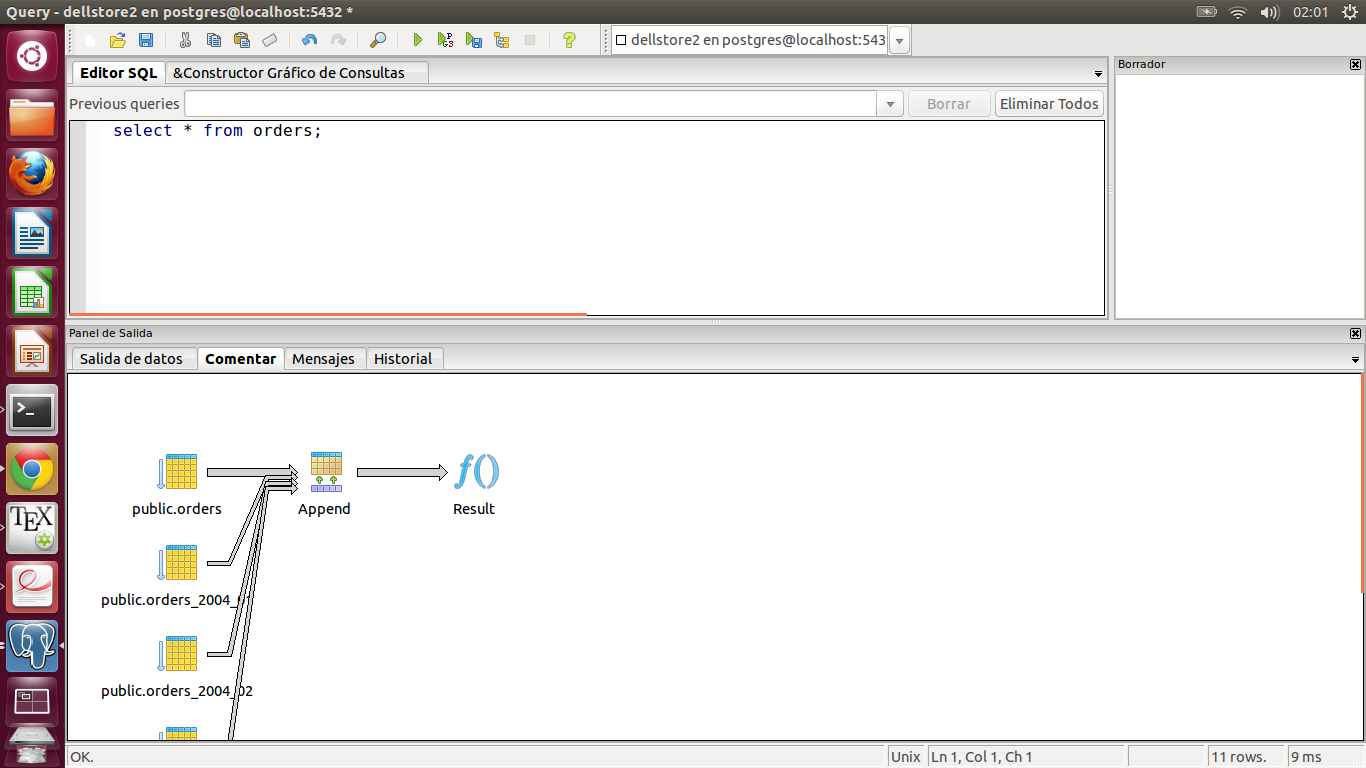
\includegraphics[scale=0.3]{imagenes/analyze_grafico_pgadmin.png}
   \caption{EXPLAIN ANALYZE gráfico en PgAdmin}\label{graf:analyze-grafico}
\end{figure}



\newpage

Ejercicios

\begin{enumerate}
\item Ejecutar las consultas relativas a dellstore2 en el analizador visual de PgAdmin.
\end{enumerate}
